%This work is licensed under the Creative Commons
%Attribution-ShareAlike 4.0 International License. To view a copy of
%this license, visit http://creativecommons.org/licenses/by-sa/4.0/ or
%send a letter to Creative Commons, PO Box 1866, Mountain View, CA
%94042, USA.

%This work is licensed under the Creative Commons
%Attribution-ShareAlike 4.0 International License. To view a copy of
%this license, visit http://creativecommons.org/licenses/by-sa/4.0/ or
%send a letter to Creative Commons, PO Box 1866, Mountain View, CA
%94042, USA.

%\documentclass[gray,handout, pdftex, 11pt]{beamer}
%\documentclass[handout, pdftex, 11pt]{beamer}

\documentclass[pdftex, 11pt]{beamer}

\usepackage[utf8]{inputenc}
\usepackage[T1]{fontenc}
\usepackage{lmodern}
%\usepackage[italian]{babel}
\usepackage{graphicx}
\usepackage{listings}
\usepackage{microtype}
\usepackage{acronym}
\usepackage{array}
\usepackage{tikz}
\usetikzlibrary{shapes, chains, scopes, shadows, positioning, arrows,
  decorations.pathmorphing, calc}

\colorlet{c1}{green!20}
\colorlet{c2}{blue!10}
\colorlet{drawColor}{black!50}
\colorlet{commentColor}{green!70!black!90}

\tikzstyle{oval}=[ellipse, align=center, drop shadow, draw=drawColor, fill=white]
\tikzstyle{rect}=[rectangle, rounded corners=2pt, align=center, drop
shadow, draw=drawColor, fill=white]
\tikzstyle{comment}=[text=commentColor,font=\itshape]
\tikzstyle{textLab}=[]
\tikzstyle{arrow}=[->, very thick, >=stealth', draw=black!80]
\tikzstyle{darrow}=[->, dash pattern=on 3pt off2pt, very thick, >=stealth', draw=black!80]
\tikzstyle{fStartEnd}=[ellipse, align=center, drop shadow, draw=drawColor, fill=white]
\tikzstyle{fInput}=[trapezium, trapezium left angle=70, trapezium right angle=110,
align=center, drop shadow, draw=drawColor, fill=white]
\tikzstyle{fProcess}=[rectangle, align=center, drop shadow, draw=drawColor, fill=white]
\tikzstyle{fSelection}=[diamond, shape aspect=3, align=center, drop
shadow, draw=drawColor, fill=white]
\tikzstyle{fOutput}=[tape, tape bend top=none, align=center, drop shadow, draw=drawColor, fill=white]
\tikzstyle{mem}=[rectangle, align=center, draw=drawColor, fill=white]
\tikzstyle{clo}=[cloud, aspect=2, align=center, drop shadow, draw=drawColor, fill=white]

\lstdefinestyle{customc}{
   language=C,
   % basicstyle=\small\ttfamily\bfseries,
   basicstyle=\ttfamily,
   keywordstyle=\color{blue}\ttfamily,
   stringstyle=\color{red}\ttfamily,
   commentstyle=\color{green}\ttfamily,
   morecomment=[l][\color{magenta}]{\#},
   % breaklines=false,
    breaklines=true, breakatwhitespace=false,
   frameround=fttt,
   frame=trBL,
   backgroundcolor=\color{yellow!20},
   numbers=left,
   stepnumber=1,    
   firstnumber=1,
   numberfirstline=true,
   numberstyle=\tiny\color{black!50},
   xleftmargin=2em,
   framexleftmargin=1.5em
   % linewidth=8cm,
}

\lstnewenvironment{cblock}[1][]
{
  \lstset{
    style=customc,
    #1
  }
}{}

\newcommand{\cfile}[2][]{
  \lstinputlisting[style=customc, #1]{#2}
}

\definecolor{links}{HTML}{2A1B81}
\hypersetup{colorlinks,linkcolor=links,urlcolor=links}

\definecolor{links}{HTML}{2A1B81}
\hypersetup{colorlinks,linkcolor=,urlcolor=links}


\mode<presentation>{
  %-------------------------1
  \usetheme{Boadilla}
  \usecolortheme{beaver}
  %-------------------------1
  %-------------------------2
  %\usetheme{Goettingen}
  %\usecolortheme{sidebartab}
  %-------------------------2
  %\useoutertheme[right]{sidebar}
  %\usefonttheme{default}
  \setbeamercovered{transparent}
  %\setbeameroption{show notes on second screen=right}
  \setbeamertemplate{navigation symbols}{}
  \setbeamertemplate{footline}{}

  \bibliographystyle{abbrv}  
  %\renewcommand\bibfont{\scriptsize}
  \setbeamertemplate{bibliography item}{\textbullet}
  \setbeamertemplate{itemize item}{\checkmark}
  \setbeamertemplate{itemize subitem}{-}
  \setbeamertemplate{enumerate items}[default]
  \setbeamertemplate{sections/subsections in toc}[square]
}

\subtitle{Logical Computational Thinking}
\institute[Tecnológico de Monterrey]{
  
\includegraphics[width=5cm]{img/logoTEC.jpg}\\[5mm]
  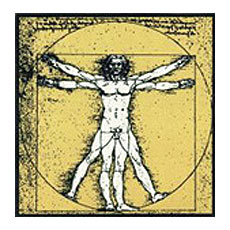
\includegraphics[width=1cm]{img/logoLEO.jpg}
  Scuola Leonardo Da Vinci (Firenze)
}

\author[Stefano Martina]{
  %\\[0.2cm]
  \textbf{Stefano MARTINA}\\
  {\small stefano.martina@gmail.com}
}

\titlegraphic{\tiny
  \href{http://creativecommons.org/licenses/by-sa/4.0/}{
\includegraphics[width=1cm]{img/logoCC.png}}
  This work is licensed under a
  \href{http://creativecommons.org/licenses/by-sa/4.0/}{Creative
    Commons Attribution-ShareAlike 4.0 International License}.}


\title[Lesson 2]{\textbf{Lesson 2 - Introduction to C language}}
\date[10/9/15]{\flushright 10 September 2015}

\begin{document}

\begin{frame}[plain]
  \titlepage
\end{frame}

\begin{frame}
  \frametitle{Review}
  \begin{center}
    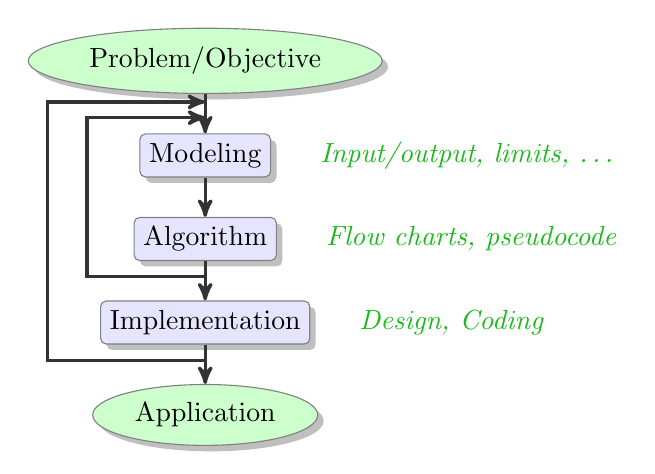
\begin{tikzpicture}[node distance=5mm]
      \node (realProb) [oval, fill=c1] {Problem/Objective};
      \node (model) [rect, fill=c2, below=of realProb] {Modeling};
      \node [comment, right=of model] {Input/output, limits, \dots};
      \draw [arrow] (realProb) -- (model);
      \node (algorithm) [rect, fill=c2, below=of model] {Algorithm};
      \node [comment, right=of algorithm] {Flow charts, pseudocode};
      \draw [arrow] (model) -- (algorithm);
      \node (implementation) [rect, fill=c2, below=of algorithm] {Implementation};
      \node [comment, right=of implementation] {Design, Coding};
      \draw [arrow] (algorithm) -- (implementation);
      \node (application) [oval, fill=c1, below=of implementation] {Application};
      \draw [arrow] (implementation) -- (application);
      \draw [arrow] ($ (implementation.south) + (0,-2mm) $) -- ++(-20mm,0) |- ($ (model.north) + (0,4mm) $);
      \draw [arrow] ($ (algorithm.south) + (0,-2mm) $) -- ++(-15mm,0) |- ($ (model.north) + (0,2mm) $);
    \end{tikzpicture}
  \end{center}
\end{frame}

\begin{frame}
  \frametitle{Model}
  \begin{center}
    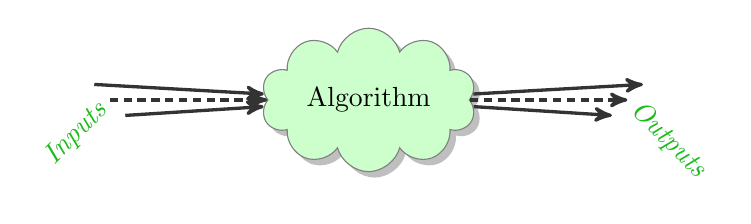
\begin{tikzpicture}[node distance=20mm]
      \node (inputs) [comment, rotate=45] {Inputs};
      \node (algorithm) [clo, fill=c1, right=of inputs] {Algorithm};
      \node (outputs) [comment, right=of algorithm, rotate=315] {Outputs};
      \draw [arrow] (inputs.north east) -- (algorithm);
      \draw [darrow] (inputs.east) -- (algorithm);
      \draw [arrow] (inputs.south east) -- (algorithm);
      \draw [arrow] (algorithm) -- (outputs.north west);
      \draw [darrow] (algorithm) -- (outputs.west);
      \draw [arrow] (algorithm) -- (outputs.south west);
    \end{tikzpicture}    
  \end{center}
\end{frame}

\begin{frame}
  \frametitle{Algorithm}
  \begin{center}
        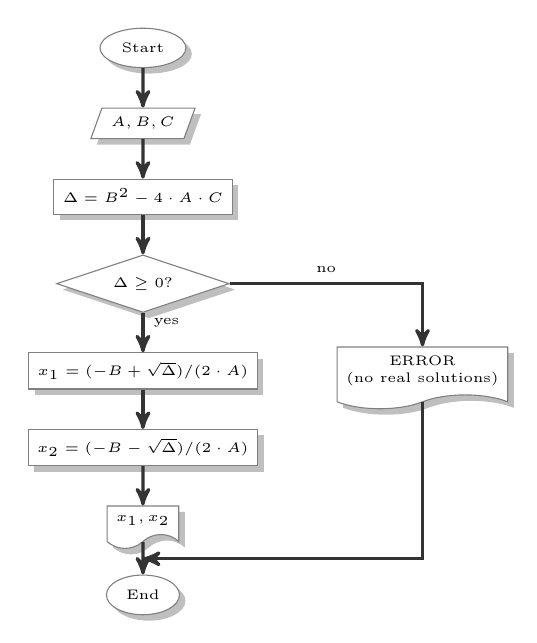
\begin{tikzpicture}[node distance=5mm, font=\tiny, auto]
      \node(start) [fStartEnd] {Start};
      \node(input) [fInput, below=of start] {$A,B,C$};
      \draw [arrow] (start) -- (input);
      \node(opD) [fProcess, below=of input] {$\Delta = B^2-4\cdot
        A\cdot C$};
      \draw [arrow] (input) -- (opD);
      \node(selection) [fSelection, below=of opD] {$\Delta\ge 0$?};
      \draw [arrow] (opD) -- (selection);
      \node(opX1T) [fProcess, below=of selection]
      {$x_1=(-B+\sqrt{\Delta})/(2\cdot A)$};
      \draw [arrow] (selection) -- node [near start] {yes} (opX1T);
      \node(opX2T) [fProcess, below=of opX1T]
      {$x_2=(-B-\sqrt{\Delta})/(2\cdot A)$};
      \draw [arrow] (opX1T) -- (opX2T);
      \node(outputErr) [fOutput, right=10mm of opX1T] {ERROR\\(no real
      solutions)};
      \draw [arrow] (selection) -| node [near start] {no} (outputErr);
      \node(output) [fOutput, below=of opX2T] {$x_1, x_2$};
      \draw [arrow] (opX2T) -- (output);
      \node(end) [fStartEnd, below=of output] {End};
      \draw [arrow] (output) -- (end);
      \draw [arrow] (outputErr) |- ($ (end.north) + (0,2mm) $);
    \end{tikzpicture}
  \end{center}
\end{frame}

\begin{frame}
  \frametitle{C language}
  \begin{figure}[h!]
    \centering
    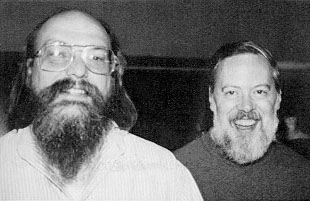
\includegraphics[width=5cm]{img/ken_n_dennis.jpg}
    \caption{Ken Thompson and Dennis Ritchie}
  \end{figure}
  \begin{block}{History}
    \begin{itemize}
    \item The language \alert{C} is developed in the 70's by Dennis Ritchie
    \item Along with the \alert{Unix} system, created by Ken Thompson and
      Dennis Ritchie in the same years
    \end{itemize}
  \end{block}
\end{frame}

\begin{frame}[fragile]
  \frametitle{Basis}
    \begin{cblock}
#include<stdio.h>  //library 

void main() {  //begin of main
  printf("Hello world!\n");
}
\end{cblock}
\cfile{../cSrc/hello_world.c}
\end{frame}
\end{document}